\section{Introduction}

The succesful finding of the, widely expected, Higgs Boson ~\cite{higgsPaperCMS,higgsPaperATLAS}
(the only scalar fundamental particle), and its $125~\mathrm{GeV}$, ligther than expected mass,
requires a high level fine tuning of the Standard Model (SM) through the
manually set properties of the now seventeen elementary particles.
This suggests an underlaying, more fundamental structure to be discovered and
a theory beyond the standard model. Other
reasons that are strongly coherent with this suggestion are: the wildly
different masses of the three different families of particles, the lack of
mass ratios predictions, open questions such as the structure of dark matter,
let alone the inclusion of gravity.

Some of the most promising hypotheses addressing the Electroweak Symmetry
Breaking (EWSB), propose that the Higgs field
emerges from a new strongly-interacting composite sector. An unavoidable
consequence from these theories, is the existance of Spin-1 vector resonances
decaying to heavy vector bosons.  Broadly speaking these resonances
fall into  two categories: electrically
charged resonances, commonly refered as $W^{\prime}$ and
neutral resonances $Z^{\prime}$. These resonances might be available at the TeV
scale ~\cite{tevscale2014}, the current LHC energy range. The question then becomes:
can experimental evidence of the existance of such resonances be found?

Vector boson resonances are a prediction of a large number
of SM extensions, including, but not limited to, the Electroweak Chiral
Lagrangian model ~\cite{echl2017}, the Little Higgs
~\cite{littlehiggs2007}, the Randall-Subdrum  model ~\cite{randall1999}, the
Minimal walking technicolor ~\cite{technicolor2007}, or models where the Higgs
is a composite pseudo-Nambu-Goldstone boson ~\cite{composite2016}.

\begin{figure}[tph]
  \centering
  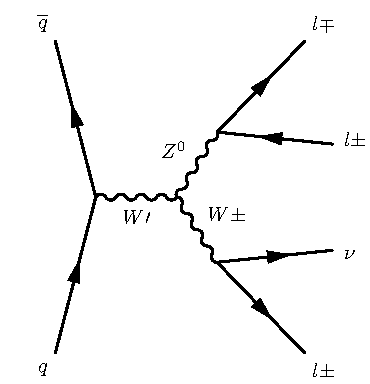
\includegraphics[width=0.4\textwidth]{fig/WprimeFeynmanDiagram.pdf}
  \caption{ Feynman Diagram of the fully leptonic decay for the
    electrically charged resonance $W^{\prime}$ to WZ.}
  \label{fig:Wprime_FeynmanDiagram}
\end{figure}

In this analysis, we test a set of theoretical models based on a phenomenological
lagrangian that contains Heavy Vector Triplets (HVT): the HVT framework, which
generalizes a large number of models predicting Spin-1 resonances ~\cite{hvt2014}.
Using two benchmarks: A weakly coupled extended gauge symmetry (referred as model A) and a
strongly coupled composite higgs scenario (model B). Further theoretical treatment of these models
is provided by Refs. ~\cite{hvt2014,modelA1980,modelB2011}. Specifically, a search
for an electrically charged resonance $W^{\prime}$ is performed. This search focuses
on the $W^{\prime}$ fully leptonic decay:
$W^{\prime}\rightarrow WZ \rightarrow \ell\nu \ell\ell$ ($\ell = e$ or $\mu$).
Despite the low branching ratio of the leptonic decay, it offers low SM backgrounds.
In this channel, the SM $Z^{0}$
boson decays to a pair of same flavoured, opposite charged leptons and the
electrically charged $W^{\pm}$ decays to a lepton and a neutrino, see Feynman diagram
on figure \ref{fig:Wprime_FeynmanDiagram}. The neutrino $\nu$ escapes
undetected and therefore needs to be reconstructed from the missing transverse
energy in the Compact Muon Solenoid (CMS) detector.

The accuracy of the MC simulations for the SM processes is then studied in a
dedicated signal-depleted control region of the phase space. A variety of
corrections on the MC samples are applied in order to account for the different
rates of efficiencies in the data reconstruction, particle identification, and
inefficiencies in the simulation of generated processes, as well as the
contribution from multiple proton-to-proton interactions occurring per bunch
crossing at the LHC accelerator.

The invariant mass for the diboson resonance candidates is
examined where a localized excess of events is expected if the resonance is
found, or otherwise, an agreement with the rates predicted by the standard model
within the statistical and systematic uncertainties will be found.
A fit to a background-only and background plus signal hypothesis is performed
through maximum likelihood estimation. Systematic uncertainties are
treated as nuisance parameters of the likelihood function.

The analysis is based on proton-proton collision data, with a center of mass
energy of $\sqrt{s}=13$ TeV collected by the CMS collaboration during the the
2016-2018 period, corresponding to an integrated luminosity of $L=137.2~fb^{-1}$.
